\documentclass[11pt]{article}
\usepackage[a4paper,margin=25mm]{geometry}
\usepackage[T1]{fontenc}
\usepackage{lmodern,microtype,amsmath,amssymb,amsthm,booktabs,graphicx,xcolor}
\usepackage[colorlinks=true,linkcolor=blue!45!black,urlcolor=blue!45!black,citecolor=blue!45!black]{hyperref}
\usepackage{enumitem,fancyhdr}
\setlist{nosep}
\pagestyle{fancy}\fancyhf{}\fancyhead[L]{\small Equal zeta functions, unequal rational planes}\fancyhead[R]{\small Shivam Gupta}\fancyfoot[C]{\thepage}
\setlength{\headheight}{14pt}
\newtheorem{theorem}{Theorem}
\newtheorem{lemma}[theorem]{Lemma}
\newtheorem{proposition}[theorem]{Proposition}
\newtheorem{corollary}[theorem]{Corollary}
\theoremstyle{remark}\newtheorem{remark}[theorem]{Remark}
\newcommand{\F}{\mathbb F}\newcommand{\PP}{\mathbb P}\newcommand{\Z}{\mathbb Z}
\title{Equal Zeta Functions, Unequal Rational Planes:\\Diagonal Cubic Fourfolds over Finite Fields}
\author{Shivam Gupta\\\small Independent Researcher\\\small\href{mailto:shivam1720406@gmail.com}{shivam1720406@gmail.com}}
\date{17 October 2026}
\begin{document}\maketitle
\begin{abstract}
Point counting compresses arithmetic geometry into Frobenius traces. We give an explicit pair of smooth diagonal cubic fourfolds for which this compression loses the existence of a rational plane. Over every finite field $k=\F_q$ of characteristic at least five with $q\equiv1\pmod3$, choose a noncube $a\in k^\times$. The coefficient patterns $(1,1,1,1,a,a^2)$ and $(1,1,a,a,a^2,a^2)$ have identical zeta functions, while their schemes of planes have respectively zero and 27 rational points. We compute both zeta functions and the complete Frobenius orbit decompositions of their 405 geometric planes. Equality persists for the zeta functions of their varieties of lines, by the established Galkin--Shinder relation. An elementary Hessian argument classifies every plane on a diagonal cubic in the stated characteristic, so the plane distinction is exhaustive. Over $\F_7$, a complete classification of diagonal fourfolds gives ten projective classes and nine zeta functions; the displayed pair is the unique collision. Reproducible exact computations comprise 150 point-count cases, 20 direct projective enumerations, 22 independent Grassmannian searches, and direct line enumeration for the displayed pair. The examples provide compact regression fixtures for arithmetic databases that must preserve incidence information beyond zeta functions.
\end{abstract}
\noindent\textbf{Keywords.} Cubic fourfolds; finite fields; rational planes; diagonal twists; Jacobi sums; zeta functions.\\
\textbf{MSC 2020.} 14G15, 14G10, 14J35, 14N20.\\
\textbf{Code and data.} \url{https://github.com/shi1720/plane-shadow}.

\section{Introduction}
A zeta function records the number of rational points over every finite extension. For a cubic fourfold, it also determines the point counts of the variety of lines. It is therefore natural to ask how much further incidence information is recoverable from these arithmetic traces. In particular, does the zeta function determine whether a cubic fourfold contains a plane over its ground field?

The answer is negative even among diagonal twists of the Fermat cubic, and even if one also supplies all point counts of the variety of lines. This paper isolates a small, explicit obstruction. Let $k=\F_q$ have characteristic at least five, let $q\equiv1\pmod3$, and choose a noncube $a\in k^\times$. Consider
\begin{align}
X_a:\quad &x_0^3+x_1^3+x_2^3+x_3^3+a x_4^3+a^2x_5^3=0,\label{eq:X}\\
Y_a:\quad &x_0^3+x_1^3+a x_2^3+a x_3^3+a^2x_4^3+a^2x_5^3=0.\label{eq:Y}
\end{align}
Both are smooth: their partial derivatives cannot vanish simultaneously at a projective point. Both become Fermat cubics over $\F_{q^3}$. Their difference is arithmetic descent, rather than geometric deformation.

Write $F_r(V)$ for the scheme of projective $r$-planes contained in $V$, and
\[
Z(V,T)=\exp\left(\sum_{m\geq1}\#V(\F_{q^m})\frac{T^m}{m}\right).
\]
The following statement combines the principal conclusions; the explicit common denominator appears in Theorem~\ref{thm:zeta}.

\begin{theorem}\label{thm:main}
For the fourfolds \eqref{eq:X}--\eqref{eq:Y},
\[
Z(X_a,T)=Z(Y_a,T),\qquad Z(F_1(X_a),T)=Z(F_1(Y_a),T),
\]
but
\[
\#F_2(X_a)(k)=0,\qquad \#F_2(Y_a)(k)=27.
\]
The plane schemes are finite \'etale of degree 405, with Frobenius cycle types
\[
F_2(X_a):3^{135},\qquad F_2(Y_a):1^{27}3^{126}.
\]
Consequently, $X_a$ and $Y_a$ are not projectively isomorphic over $k$.
\end{theorem}

The main contribution is the explicit comparison between arithmetic traces and the descent of actual linear subspaces. The counting tools are classical. Our proofs separate those tools from the finite combinatorics that creates the collision, and our computations test the two sides independently. Figure~\ref{fig:workflow} summarizes this separation.

\begin{figure}[ht]
\centering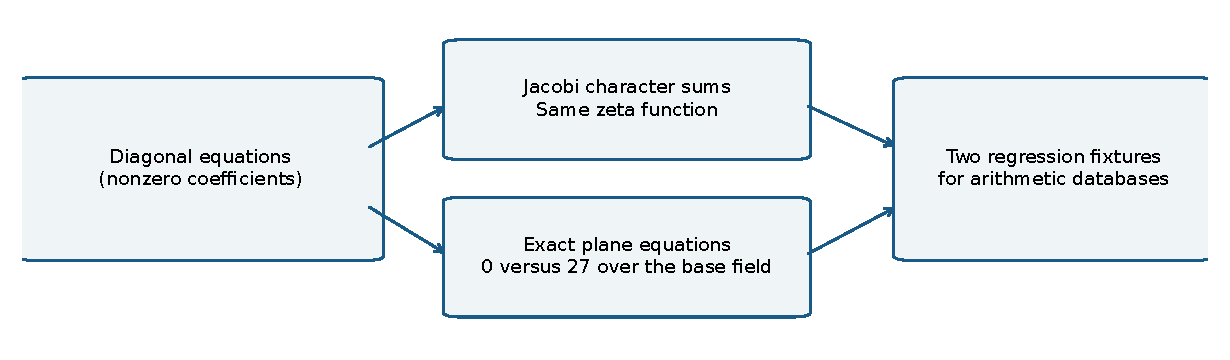
\includegraphics[width=\linewidth]{figures/workflow.pdf}
\caption{Two exact calculations on the same equations. The point-count invariant agrees, while plane descent distinguishes the fourfolds. Neither branch is inferred from the output of the other.}\label{fig:workflow}
\end{figure}

\section{Relation to established work}
Weil's treatment of equations over finite fields supplies the character-sum method and the extension-field lifting relation underlying diagonal zeta functions~\cite{weil}. Gouv\^ea and Yui develop diagonal twists and their arithmetic systematically~\cite{gy}. We specialize that established framework to six cubic terms and retain the coefficient-class multiplicities needed to compare zeta functions with plane descent. We do not propose a new point-counting method or a replacement for twisted Jacobi sums.

The geometric plane configuration is also classical. Degtyarev, Itenberg, and Ottem study planes on complex cubic fourfolds and characterize the Fermat cubic as the unique complex example with 405 planes~\cite{dio}. That extremal theorem is not used in positive characteristic here: Section~\ref{sec:planes} gives a direct Hessian proof for diagonal cubics in characteristic different from two and three. Shioda and Katsura place Fermat varieties in the broader study of algebraic cycles and their inductive structure~\cite{sk}.

Auel, Kulkarni, Petok, and Weinbaum compute a census of cubic fourfolds over $\F_2$, including zeta functions and line and plane counts~\cite{akpw}. Our examples lie in a different characteristic and form a much smaller family. Their census already makes clear the value of storing these invariants together; we provide a symbolic family and a minimal diagonal collision illustrating why the incidence fields must remain separate. Addington and Auel use finite-field point counting to study Noether--Lefschetz generality~\cite{aa}; our result concerns rational representatives by planes, not the validity of their cohomological method.

The equality for varieties of lines is an application of the Galkin--Shinder point-count relation, in the form given by Debarre, Laface, and Roulleau~\cite{dlr}. It is a consequence of the common zeta function, not a separate new formula. The contribution claimed here is the explicit pair, its complete plane descent calculation, the ten-class computation over $\F_7$, and the reproducible comparison. We make no priority claim for the general phenomenon that a zeta function is an incomplete geometric invariant.

\section{The character signature of a diagonal cubic}
Fix a primitive complex cube root of unity $\zeta$ and a cubic character $\chi:k^\times\to\{1,\zeta,\zeta^2\}$, extended by $\chi(0)=0$. Choose its orientation so that $\chi(a)=\zeta$. For
\[
V_{\boldsymbol c}:\quad \sum_{i=0}^5 c_i x_i^3=0,\qquad c_i\in k^\times,
\]
write $\chi(c_i)=\zeta^{d_i}$, with $d_i\in\Z/3\Z$, and put
\begin{equation}\label{eq:signature}
S=\sum_i d_i,\qquad b_j=\#\left\{I\subset\{0,\ldots,5\}:|I|=3,\quad S+\sum_{i\in I}d_i=j\right\}.
\end{equation}
Complementation of $I$ negates its residue, so $b_1=b_2$ and $b_0+2b_1=20$.

Let $\psi$ be a nontrivial additive character and set
\[
G_1=\sum_{u\in k^\times}\chi(u)\psi(u),\qquad
G_2=\sum_{u\in k^\times}\chi(u)^2\psi(u),\quad
\alpha=G_1^6/q,\quad\beta=G_2^6/q.
\]
Because $-1$ is a cube, $G_1G_2=q$. The Gauss--Jacobi identity gives
\[
J=\sum_{u\in k}\chi(u)\chi(1-u)\in\Z[\zeta],\qquad
\alpha=qJ^2,\quad \beta=q\overline J^{\,2},\quad J\overline J=q.
\]
In particular $\beta=\overline\alpha$ and $\alpha\beta=q^4$. These are the standard identities for cubic characters~\cite{weil,gy}.

\begin{proposition}\label{prop:points}
With the preceding notation,
\begin{equation}\label{eq:count}
\#V_{\boldsymbol c}(k)=1+q+q^2+q^3+q^4+
\alpha\zeta^{-S}+\beta\zeta^{-2S}+q^2(b_0-b_1).
\end{equation}
For extension degree $m$, replace $q$ by $q^m$, $\alpha,\beta$ by $\alpha^m,\beta^m$, and each $d_i$ by $m d_i$ in \eqref{eq:signature} and \eqref{eq:count}.
\end{proposition}
\begin{proof}
For $t\ne0$, counting the three cube roots of each nonzero cube gives
\[
\sum_{x\in k}\psi(t c_i x^3)=\chi(tc_i)^{-1}G_1+\chi(tc_i)^{-2}G_2.
\]
Additive orthogonality expresses the number of affine zeroes as $q^{-1}$ times the sum over $t\in k$ of the product of these six expressions. The $t=0$ term is $q^5$. In the expansion for $t\ne0$, a term survives summation precisely when its total character exponent is divisible by three. The six exponents belong to $\{1,2\}$; the number of ones must therefore be zero, three, or six.

The two constant choices give $G_1^6\zeta^{-S}$ and $G_2^6\zeta^{-2S}$. For a three-element set $I$ of positions carrying exponent one, the coefficient phase is
\[
\zeta^{-\sum_{i\in I}d_i-2\sum_{i\notin I}d_i}
=\zeta^{S+\sum_{i\in I}d_i}.
\]
Its Gauss product is $G_1^3G_2^3=q^3$. Removing the affine origin and dividing by $q-1$ yields the projective count. Since $b_1=b_2$, the balanced phase sum is $b_0+b_1\zeta+b_2\zeta^2=b_0-b_1$.

Over $k_m=\F_{q^m}$, use $\chi_m=\chi\circ N_{k_m/k}$ and $\psi_m=\psi\circ\operatorname{Tr}_{k_m/k}$. On a base-field coefficient, $\chi_m(c_i)=\chi(c_i)^m$. The Hasse--Davenport lifting relation gives $G_{e,m}=(-1)^{m-1}G_e^m$. Taking sixth powers removes the sign, giving $G_{1,m}^6/q^m=\alpha^m$ and likewise for $\beta$. Applying the base-field calculation over $k_m$ proves the assertion.
\end{proof}

For $X_a$ the class vector is $(0,0,0,0,1,2)$. The three-subsets contain neither exceptional position, both positions, just the class-one position, or just the class-two position. The corresponding counts are $4,4,6,6$, giving $(b_0,b_1,b_2)=(8,6,6)$ and $S=0$.
For $Y_a$ the vector is $(0,0,1,1,2,2)$. Eight three-subsets select one position from each class and have residue zero. The remaining twelve split equally between residues one and two. Thus the same signature occurs.

If $3\mid m$, both vectors become zero and have signature $(0;20,0,0)$. Otherwise the signature remains $(0;8,6,6)$. Proposition~\ref{prop:points} therefore gives, for both fourfolds,
\begin{equation}\label{eq:allcounts}
N_m=\sum_{j=0}^4q^{jm}+\alpha^m+\beta^m+
q^{2m}\begin{cases}20,&3\mid m,\\2,&3\nmid m.\end{cases}
\end{equation}
This proves equality over all extensions, not only over the finite set of fields used in the experiments.

\begin{theorem}\label{thm:zeta}
Put $A=q(J^2+\overline J^{\,2})\in\Z$. The common zeta function of $X_a,Y_a$ is
\begin{equation}\label{eq:zeta}
\frac{1}{(1-T)(1-qT)(1-q^2T)^9
(1+q^2T+q^4T^2)^6(1-AT+q^4T^2)(1-q^3T)(1-q^4T)}.
\end{equation}
\end{theorem}
\begin{proof}
The periodic term in \eqref{eq:allcounts} equals
$q^{2m}(8+6\zeta^m+6\zeta^{2m})$.
Exponentiating its generating series gives
$(1-q^2T)^{-8}(1+q^2T+q^4T^2)^{-6}$.
The baseline contributes the five projective-space factors, and $\alpha,\beta$ contribute $1-AT+q^4T^2$. Combining the two factors at $q^2$ yields \eqref{eq:zeta}.
\end{proof}

\section{Every plane is a coordinate pairing}\label{sec:planes}
A pairing of the six coordinate positions into three unordered pairs produces planes on a diagonal cubic. The following lemma shows that, in our characteristic range, it produces every plane. It also supplies a short proof that does not transfer a characteristic-zero classification to a finite field.

\begin{lemma}[Plane classification]\label{lem:planes}
Let $K$ be any field of characteristic different from two and three, and let $c_0,\ldots,c_5\in K^\times$. Every $K$-plane in $\sum c_i x_i^3=0$ is obtained by a partition into pairs $\{i_r,j_r\}$ and equations
\[
x_{j_r}=u_r x_{i_r},\qquad u_r^3=-c_{i_r}/c_{j_r},\qquad r=1,2,3.
\]
Different pairings and root choices give different planes. Over an algebraic closure there are $15\cdot3^3=405$ planes, and their scheme is reduced.
\end{lemma}
\begin{proof}
Restrict the coordinate functions to the three-dimensional vector space underlying a plane. Choose three independent restrictions and rename them $t_0,t_1,t_2$. The remaining restrictions are linear forms $L_0,L_1,L_2$. The cubic identity on the plane is
\begin{equation}\label{eq:cubeidentity}
u_0t_0^3+u_1t_1^3+u_2t_2^3+
 v_0L_0^3+v_1L_1^3+v_2L_2^3=0,
\end{equation}
where all six coefficients are nonzero. Write $L=Bt$. The determinant of the Hessian of the first sum is
$6^3u_0u_1u_2t_0t_1t_2$, a nonzero polynomial. The determinant of the Hessian of the second sum is
\[
6^3\det(B)^2v_0v_1v_2L_0L_1L_2.
\]
Equation~\eqref{eq:cubeidentity} implies that these determinants agree up to sign. Hence $B$ is invertible and $L_0L_1L_2$ is a nonzero scalar multiple of $t_0t_1t_2$. Unique factorization forces the three $L_i$ to be nonzero multiples of distinct $t_j$. Matching coefficients now gives exactly the stated pairing equations. Each of the three proportionality classes has exactly two coordinate restrictions, so the pairing is unique.

There are 15 perfect matchings of six positions and three distinct roots for each ratio over an algebraic closure. To check reducedness, use a Grassmannian chart with the three selected coordinates as free coordinates. At a pairing plane, vary the three remaining linear forms by arbitrary first-order linear forms. The linearized cubic restriction is a nonzero diagonal scaling of
$\sum_i t_i^2\delta L_i$. The nine monomials $t_i^3$ and $t_i^2t_j$ for $i\ne j$ are distinct, so this linear map is injective. The tangent space of the plane scheme is zero at every geometric point. A projective scheme with this finite geometric support and zero tangent spaces is finite and reduced, proving the claim.
\end{proof}

\begin{proposition}\label{prop:descent}
For $k=\F_q$ in Theorem~\ref{thm:main}, let $n_j$ be the number of coefficients in cubic class $j$. Then
\begin{equation}\label{eq:planeformula}
\#F_2(V_{\boldsymbol c})(k)=
\begin{cases}
27\displaystyle\prod_{j=0}^2(n_j-1)!!,&\text{all }n_j\text{ are even},\\
0,&\text{otherwise},
\end{cases}
\end{equation}
where $(-1)!!=1$. For $X_a,Y_a$ the plane counts over $k_m$ are respectively
\[
\begin{array}{c|cc}
&3\nmid m&3\mid m\\\hline
X_a&0&405\\
Y_a&27&405.
\end{array}
\]
Their plane-scheme zeta functions are
\begin{equation}\label{eq:planezeta}
Z(F_2(X_a),T)=(1-T^3)^{-135},\qquad
Z(F_2(Y_a),T)=(1-T)^{-27}(1-T^3)^{-126}.
\end{equation}
\end{proposition}
\begin{proof}
Because $-1$ is a cube, a ratio $-c_i/c_j$ has a cube root in $k$ exactly when the coefficients have the same cubic class. In that case it has three roots. Thus each class must have even size, there are $(n_j-1)!!$ pairings within class $j$, and every complete matching contributes 27 planes. Lemma~\ref{lem:planes} proves exhaustiveness.

The multiplicities of $X_a$ are $(4,1,1)$ and those of $Y_a$ are $(2,2,2)$. For $3\nmid m$, multiplication by $m$ permutes the two nonzero classes; for $3\mid m$ all coefficients are cubes in $k_m$. This gives the table. All geometric planes are defined over $k_3$, so Frobenius orbits have lengths one or three. The base-field counts give $3^{135}$ and $1^{27}3^{126}$. The tangent-space calculation makes the plane schemes finite \'etale over the finite field, and the orbit formula for a finite \'etale scheme gives \eqref{eq:planezeta}.
\end{proof}

\begin{figure}[ht]
\centering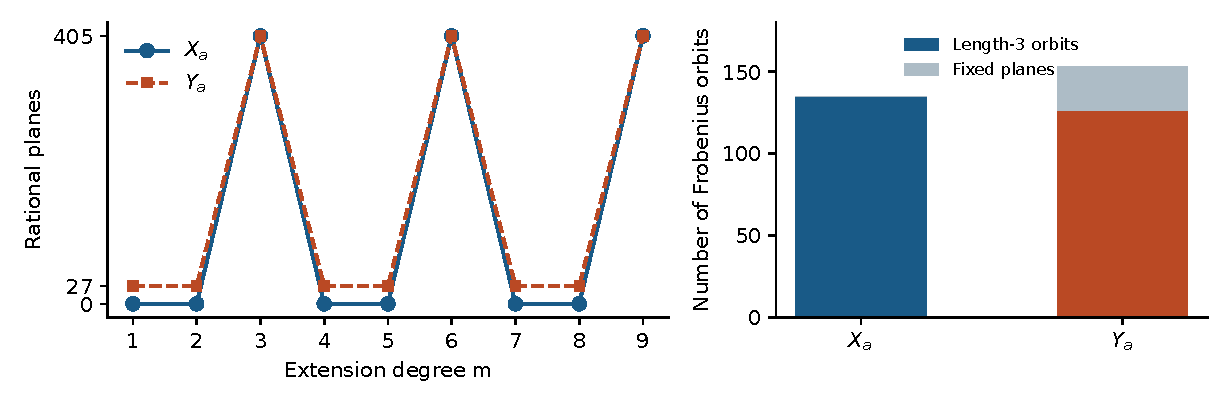
\includegraphics[width=\linewidth]{figures/plane_descent.pdf}
\caption{Plane descent for the pair. Left: plane counts over extensions depend on the degree modulo three. Right: the two actions have the same 405 geometric planes but different numbers of fixed points and length-three orbits. The connecting lines on the left are visual guides between integer degrees.}\label{fig:descent}
\end{figure}

\section{Lines do not remove the ambiguity}
For a smooth cubic fourfold $V/k$, the established Galkin--Shinder relation implies~\cite[\S2.3]{dlr}
\begin{equation}\label{eq:lines}
\#F_1(V)(k_m)=\frac{N_m(V)^2+N_{2m}(V)-2(1+q^{4m})N_m(V)}{2q^{2m}}.
\end{equation}
Substitution of \eqref{eq:allcounts} proves the second zeta-function equality in Theorem~\ref{thm:main}. Thus even all point counts of both the fourfold and its line variety fail to determine the existence of a rational plane. This conclusion uses the line variety only as an arithmetic invariant; it does not assert that its full incidence structure is identical for the pair.

For the explicit base-field example, choose $q=7$ and $a=3$, so $a^2=2$. With $\chi(3)=\zeta$ one obtains $J=-1-3\zeta$, hence $A=-91$. The quadratic factor in \eqref{eq:zeta} is $1+91T+2401T^2$. Table~\ref{tab:case} lists the first three extension counts.
\begin{table}[ht]\centering
\caption{Exact values for $X_3,Y_3$ over $\F_7$. Point counts and line counts agree in every extension by proof; the displayed finite-field point counts are directly computed here. Line counts use \eqref{eq:lines}; the base-field value is also independently enumerated.}\label{tab:case}
\begin{tabular}{rrrrr}\toprule
$m$&Points on either fourfold&Lines on either&Planes on $X_3$&Planes on $Y_3$\\\midrule
1&2,808&2,943&0&27\\
2&5,893,182&6,315,921&0&27\\
3&13,884,013,683&14,680,153,260&405&405\\\bottomrule
\end{tabular}
\end{table}

\section{A complete diagonal classification over $\F_7$}\label{sec:census}
A useful distinction is between labeled coefficient vectors, diagonal presentations, and projective equivalence classes. There are $3^6=729$ labeled cubic-class vectors. Changing coordinates by nonzero diagonal scalings removes cube factors from coefficients; permutation of coordinates forgets labels. Multiplication of the defining equation by a nonzero scalar cyclically shifts all three classes. Thus a candidate class is a triple $(n_0,n_1,n_2)$ summing to six, modulo cyclic rotation. There are ten such triples.

These are also the projective equivalence classes, not merely a chosen presentation quotient. Indeed, the Hessian determinant of a diagonal cubic is a nonzero scalar times $x_0\cdots x_5$. A projective linear equivalence must preserve this union of coordinate hyperplanes, because Hessian determinants transform by a nonzero scalar and change of coordinates. It is therefore monomial. The preceding cube scalings, permutations, and common scalar account for every such equivalence.

For a signature $(S;b_0,b_1,b_1)$, Proposition~\ref{prop:points} yields the middle denominator
\begin{equation}\label{eq:generalP4}
P_4(T)=(1-q^2T)^{b_0+1}(1+q^2T+q^4T^2)^{b_1}
\bigl(1-A_ST+q^4T^2\bigr),
\quad A_S=\alpha\zeta^{-S}+\beta\zeta^{-2S}.
\end{equation}
It has degree 23, including the hyperplane-square class. At $q=7$,
\[
(A_0,A_1,A_2)=(-91,14,77).
\]
The three quadratics have distinct traces and are distinct from the factors with roots $q^2$, $q^2\zeta$, and $q^2\zeta^2$. Consequently equality of these polynomials is equivalent to equality of $S$ and $b_0$ in the table below.

\begin{table}[ht]\centering
\caption{All ten projective classes of diagonal cubic fourfolds over $\F_7$. The common zeta function occurs precisely in the two marked rows. A cyclic rotation represents the same projective class.}\label{tab:census}
\begin{tabular}{crrrr}\toprule
$(n_0,n_1,n_2)$&$S$&$(b_0,b_1,b_2)$&$\#V(\F_7)$&$\#F_2(V)(\F_7)$\\\midrule
$(0,0,6)$&0&$(20,0,0)$&3690&405\\
$(0,1,5)$&2&$(0,10,10)$&2388&0\\
$(0,2,4)$&1&$(12,4,4)$&3207&81\\
$(0,3,3)$&0&$(2,9,9)$&2367&0\\
$(0,4,2)$&2&$(12,4,4)$&3270&81\\
$(0,5,1)$&1&$(0,10,10)$&2325&0\\
$\boldsymbol{(1,1,4)}$&0&$\boldsymbol{(8,6,6)}$&\textbf{2808}&\textbf{0}\\
$(1,2,3)$&2&$(6,7,7)$&2829&0\\
$(1,3,2)$&1&$(6,7,7)$&2766&0\\
$\boldsymbol{(2,2,2)}$&0&$\boldsymbol{(8,6,6)}$&\textbf{2808}&\textbf{27}\\\bottomrule
\end{tabular}
\end{table}

\begin{corollary}\label{cor:unique}
Over $\F_7$ there are ten projective equivalence classes of smooth diagonal cubic fourfolds and nine zeta functions. The unique collision is the pair of Theorem~\ref{thm:main}.
\end{corollary}
The result follows from the exhaustive triple list and the factor comparison in \eqref{eq:generalP4}. It is a classification within the diagonal family, not within all smooth cubic fourfolds. The same nine-polynomial pattern is verified at the other ten primes in the computational protocol; the paper does not need a classification theorem for every prime power.

\begin{figure}[ht]
\centering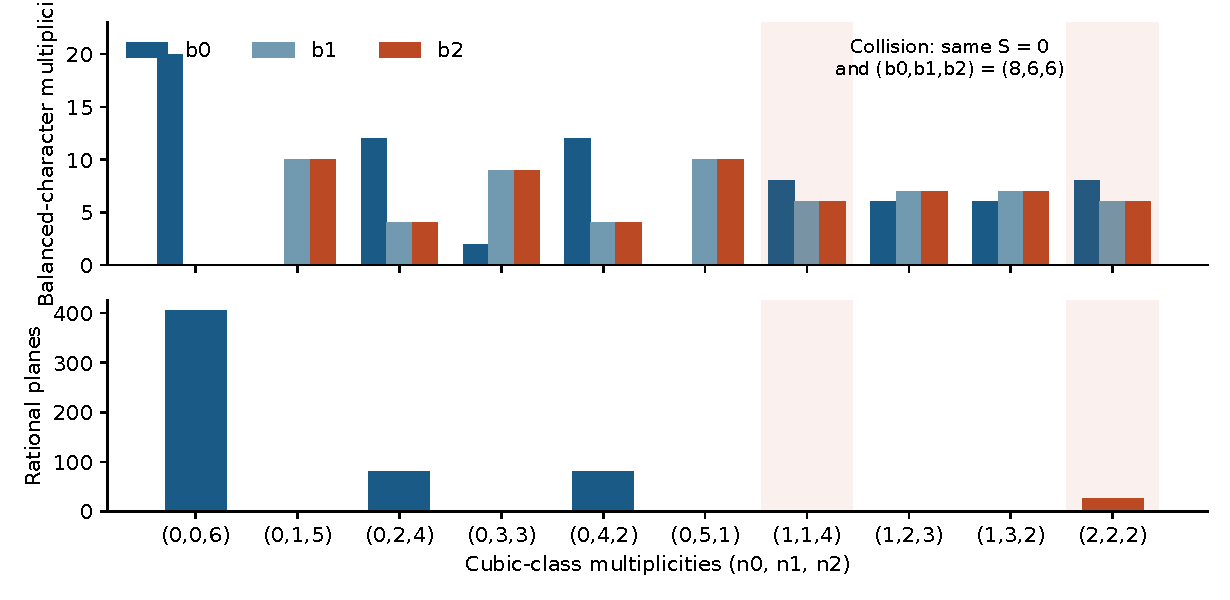
\includegraphics[width=\linewidth]{figures/twist_census.pdf}
\caption{The ten diagonal classes. The upper panel records the balanced-character multiplicities; the lower panel records rational planes. Shading marks the two rows with equal complete signatures but different plane counts. For the other rows the value of $S$ in Table~\ref{tab:census} must also be retained when comparing zeta functions.}\label{fig:census}
\end{figure}

\section{Reproducible exact computations}\label{sec:experiments}
The computations corroborate the algebraic proof and provide inspectable examples. They are finite deterministic checks, not statistical evidence for a conjecture. The core Python implementation uses only the standard library and arbitrary-precision integers. Figure generation uses Matplotlib; the independent plane search is C++17.

\paragraph{Point counting without character sums.}
For each coefficient $c$, compute the histogram $H_c(y)=\#\{x:c x^3=y\}$. Starting from the delta mass at zero, convolve six histograms using the additive group of the finite field. If the final zero entry is $M$, return $(M-1)/(q-1)$. This calculation uses neither Jacobi sums nor the signature in \eqref{eq:signature}. Extension fields use polynomial bases with moduli
\[
\F_{7^2}:u^2+1,\quad \F_{7^3}:u^3+2,\quad
\F_{13^2}:u^2+2,\quad \F_{19^2}:u^2+1.
\]
Each modulus is checked for absence of a base-field root, which proves irreducibility in degrees two and three. Addition and multiplication use exact modular arithmetic.

The protocol evaluates all ten class representatives at the primes
\[
7,13,19,31,37,43,61,67,73,79,97,
\]
and in the four extension fields above: 150 cases in total. Every value agrees with Proposition~\ref{prop:points}. A separate oracle enumerates projective points by fixing the last nonzero coordinate to one. It verifies all ten classes over $\F_7$ and $\F_{13}$, giving 20 full projective enumerations.

\paragraph{Plane verification independent of the pairing formula.}
The C++ program searches every reduced-row-echelon chart of $\operatorname{Gr}(3,6)(\F_p)$ and substitutes the resulting three-dimensional subspace into the cubic. There are twenty pivot patterns. It first enumerates the possible rows and retains only those for which the pure-cube coefficient vanishes. It then tests all products of retained rows against the six mixed coefficients and the coefficient of $t_0t_1t_2$. Since $3$ and $6$ are invertible, these ten conditions are exactly the vanishing of the restricted cubic. Every subspace has one reduced-row-echelon representative, so this is exhaustive, with algebraic pruning rather than a traversal of every unpruned matrix.

The search covers all ten classes over $\F_7$ and $\F_{13}$ and the two collision classes over $\F_{19}$. For each input its chart sizes sum to the independent Gaussian-binomial count
\[
\#\operatorname{Gr}(3,6)(\F_p)=
\prod_{i=0}^2\frac{p^{6-i}-1}{p^{3-i}-1}.
\]
For $p=7,13,19$ these totals are respectively $48{,}177{,}200$, $11{,}561{,}414{,}060$, and $341{,}607{,}982{,}520$. These are covered search spaces, not counts of executed full-subspace tests. The raw CSV separately records the much smaller numbers of row combinations surviving pure-cube pruning. All 22 resulting plane counts agree with \eqref{eq:planeformula}.

\begin{table}[ht]\centering
\caption{Executed checks. The units differ by row and are not independent samples. Every check passed.}\label{tab:checks}
\begin{tabular}{lr}\toprule
Check&Count\\\midrule
Labeled cubic-class vectors, signature and matching comparison&729\\
Histogram point counts against the character formula&150\\
Independent direct projective enumerations&20\\
Independent exhaustive Grassmannian searches&22\\
Plane matrices checked by polynomial substitution and RREF uniqueness&6,534\\
Independent base-field line enumerations for $X_3,Y_3$&2\\
Exact middle-polynomial classifications at distinct primes&11\\\bottomrule
\end{tabular}
\end{table}

For every class at the eleven base primes, the pairing routine also produces explicit plane matrices. A separate ordered-tensor expansion checks their cubic restrictions, and row reduction checks uniqueness. The total is 6,534 matrices. This verifies the constructive output; completeness is supplied independently by the Hessian proof and, on the smaller fields, by the Grassmannian search.

A further RREF search on $\operatorname{Gr}(2,6)(\F_7)$ directly enumerates all lines on the two displayed fourfolds and returns 2,943 for each, independently checking the base-field consequence of \eqref{eq:lines}.

The protocol file was fixed before the main run, but was not publicly preregistered. Its SHA-256 is recorded in \texttt{results/summary.json}. Raw outputs contain field sizes, moduli, class representatives, exact counts, and wall-clock timings. Timings are descriptive only; no competitive performance claim is made. The protocol, equations, source, and outputs permit independent reproduction without a proprietary computer algebra system.

\section{Implications, scope, and further questions}
The distinction is between a cohomological trace invariant and descent of specified geometric representatives. A Frobenius-invariant cycle class need not be represented by a single rational plane. The common middle denominator contains nine copies of the eigenvalue $q^2$, including the hyperplane-square class, even though $X_a$ has no rational plane. This is consistent with the Tate conjecture: the conjecture concerns cycle classes, not a requirement that each invariant class have a plane representative.

There is a concrete computational use. A database should store a zeta function as an invariant and a possible search key, together with separate equations, equivalence certificates, and incidence fields. Our pair is a small regression fixture: any routine that transfers rational-plane existence solely across matching zeta functions must fail on it. Recording the plane-scheme zeta function or simply the base-field plane count distinguishes the two inputs immediately. Recording more extension point counts of the fourfold cannot repair that loss, since the entire sequences already agree.

The practical software setting includes arithmetic census pipelines and computer algebra environments. SageMath provides exact scheme point-count interfaces~\cite{sage}; the published cubic census includes a substantial reusable codebase~\cite{akpw}. The present artifact supplies deliberately small inputs for validating data integration around such calculations. A possible product is a verification component for scientific databases, but customer demand, market size, revenue, and patentability are not established by this mathematics. The result supports a reproducible software capability, not a commercial-performance claim.

The scope is restricted. Characteristic two is excluded by the Hessian argument and has different Fermat geometry; characteristic three makes the displayed diagonal forms singular. We require $q\equiv1\pmod3$ to retain three base-field cubic classes. Over extensions of degree divisible by three the plane distinction disappears. We do not infer different rationality, different geometric plane configurations, or nonisomorphism of the unpolarized varieties of lines. The $\F_7$ classification covers only diagonal fourfolds.

Several precise questions remain. For higher even-dimensional diagonal cubics, which collisions of the analogous character signatures change the descent of maximal linear spaces? For general cubic fourfolds, how much additional information beyond the zeta function is needed to predict their plane schemes? Can incidence-refined census records identify families with common cohomological traces but different descent of other low-degree surfaces? These questions retain the separation between cycle classes and actual subvarieties exhibited by the present pair.

\section{Conclusion}
The fourfolds $X_a$ and $Y_a$ agree in all finite-extension point counts, as do their varieties of lines, but their rational-plane counts are zero and 27. A complete plane classification and a character-signature calculation explain both the agreement and the difference. Over $\F_7$ this is the unique zeta collision among ten diagonal projective classes. The accompanying exact implementations make the example available as a verifiable test of the geometric information preserved by arithmetic computations.

\paragraph{Availability.}
The source, protocol, raw results, figure scripts, and manuscript are available at \url{https://github.com/shi1720/plane-shadow}. The paper is a research manuscript; no peer-review acceptance is asserted. All finite computations described in Section~\ref{sec:experiments} were executed. The infinite-extension assertions are consequences of the proofs.

\begin{thebibliography}{9}
\bibitem{weil} Andr\'e Weil. Numbers of solutions of equations in finite fields. \emph{Bulletin of the American Mathematical Society} 55 (1949), 497--508. \href{https://doi.org/10.1090/S0002-9904-1949-09219-4}{doi:10.1090/S0002-9904-1949-09219-4}.
\bibitem{gy} Fernando Q. Gouv\^ea and Noriko Yui. \emph{Arithmetic of Diagonal Hypersurfaces over Finite Fields}. London Mathematical Society Lecture Note Series 209. Cambridge University Press, 1995. \href{https://doi.org/10.1017/CBO9780511526060}{doi:10.1017/CBO9780511526060}.
\bibitem{dio} Alex Degtyarev, Ilia Itenberg, and John Christian Ottem. Planes in cubic fourfolds. \emph{Algebraic Geometry} 10 (2023), no. 2, 228--258. \href{https://doi.org/10.14231/ag-2023-007}{doi:10.14231/ag-2023-007}.
\bibitem{sk} Tetsuji Shioda and Toshiyuki Katsura. On Fermat varieties. \emph{Tohoku Mathematical Journal} 31 (1979), 97--115. \href{https://doi.org/10.2748/tmj/1178229881}{doi:10.2748/tmj/1178229881}.
\bibitem{akpw} Asher Auel, Avinash Kulkarni, Jack Petok, and Jonah Weinbaum. A census of cubic fourfolds over $\F_2$. \emph{Mathematics of Computation} 94 (2025), 2089--2112. \href{https://doi.org/10.1090/mcom/4010}{doi:10.1090/mcom/4010}. Code: \url{https://github.com/JonahWeinbaum/cubic-fourfolds}.
\bibitem{aa} Nicolas Addington and Asher Auel. Some non-special cubic fourfolds. \emph{Documenta Mathematica} 23 (2018), 637--651. \href{https://doi.org/10.4171/DM/628}{doi:10.4171/DM/628}.
\bibitem{dlr} Olivier Debarre, Antonio Laface, and Xavier Roulleau. Lines on cubic hypersurfaces over finite fields. In \emph{Geometry over Nonclosed Fields}, Simons Symposia, Springer, 2017, 19--51. Corrected version: \href{https://arxiv.org/abs/1510.05803v5}{arXiv:1510.05803v5} (2021).
\bibitem{sage} The Sage Developers. Schemes: \texttt{count\_points}. \emph{SageMath Reference Manual}. \url{https://doc.sagemath.org/html/en/reference/schemes/sage/schemes/generic/scheme.html}. Accessed 17 October 2026.
\end{thebibliography}
\clearpage
\appendix
\section{Reproduction map}
From the repository root, run:
\begin{verbatim}
python3 experiments/run.py
python3 experiments/classify.py
c++ -O2 -std=c++17 tests/grassmannian.cpp -o /tmp/plane-search
/tmp/plane-search results/grassmannian.csv
c++ -O2 -std=c++17 tests/lines.cpp -o /tmp/line-search
/tmp/line-search results/lines.csv
python3 experiments/verify.py
python3 experiments/figures.py
cd paper && tectonic main.tex
\end{verbatim}
The computational checks require only Python's standard library and a C++17 compiler. Figure regeneration additionally requires Matplotlib. Compilation requires Tectonic and its usual TeX resources. The verifier compares every Grassmannian result to the separately implemented pairing count and checks the chart coverage against Gaussian binomial coefficients.

\begin{center}\small
\begin{tabular}{ll}\toprule
Path&Purpose\\\midrule
\texttt{src/plane\_shadow.py}&Field arithmetic, counts, characters, planes\\
\texttt{tests/independent.py}&Projective enumeration and substitution\\
\texttt{tests/grassmannian.cpp}&Complete RREF search with pruning\\
\texttt{experiments/protocol.json}&Finite grids and exact field definitions\\
\texttt{results/point\_counts.csv}&150 actual/formula comparisons\\
\texttt{results/grassmannian.csv}&22 independent plane searches\\
\texttt{results/zeta\_classification.json}&Exact degree-23 middle polynomials\\
\texttt{results/case\_study.json}&Extension values and line-count consequences\\\bottomrule
\end{tabular}
\end{center}
\end{document}
